%++++++++++++++++++++++++++++++++
\cscschapter{Cooperating Threads}
%++++++++++++++++++++++++++++++++

%%%%%%%%%%%%%%%%%%%%%%%%%%%%%%%%%%%%%%%%%%%%
\begin{frame}[fragile]{The Need Cooperation Between Threads}
%%%%%%%%%%%%%%%%%%%%%%%%%%%%%%%%%%%%%%%%%%%%
    \centering
    Most algorithms do not lend themselves to trivial parallelization like our \axpy example

%----------------------------
    \begin{code}{reductions : e.g. dot product}
        \begin{lstlisting}[style=boxcudatiny]
int dot(int *x, int *y, int n){
  int sum = 0.;
  for(auto i=0; i<n; ++i)
    sum += x[i]*y[i];
  return sum;
}
        \end{lstlisting}
    \end{code}
%----------------------------
\vspace{-7pt}
%----------------------------
        \begin{code}{scan : e.g. prefix sum}
            \begin{lstlisting}[style=boxcudatiny]
void prefix_sum(int *x, int n){
  for(auto i=1; i<n; ++i)
    x[i] += x[i-1];
}
        \end{lstlisting}
    \end{code}
%----------------------------
\vspace{-7pt}
%----------------------------
    \begin{code}{fusing piplined stencil loops : e.g. apply blur kernel twice}
        \begin{lstlisting}[style=boxcudatiny]
void twice_blur(float *in, float *out, int n){
  float buff[n];
  for(auto i=1; i<n-1; ++i)
    buff[i] = 0.25f*(in[i-1]+in[i+1]+2f*in[i]);
  for(auto i=2; i<n-2; ++i)
    out[i] = 0.25f*(buff[i-1]+buff[i+1]+2f*buff[i]);
}
        \end{lstlisting}
    \end{code}

\end{frame}

%%%%%%%%%%%%%%%%%%%%%%%%%%%%%%%%%%%%%%%%%%%%
\begin{frame}[fragile]{Block-Level Synchronization}
%%%%%%%%%%%%%%%%%%%%%%%%%%%%%%%%%%%%%%%%%%%%
    \begin{columns}[T]
        \begin{column}{0.3\textwidth}
            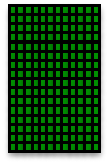
\includegraphics[width=\textwidth]{./images/smx.pdf}
        \end{column}

        \begin{column}{0.7\textwidth}
            \begin{info}{}
            CUDA provides mechanisms for cooperation between \emph{threads in a thread block}.
            \begin{itemize}
                \item All threads in a block run on the same SMX
                \item Resources for synchronization are at SMX level
                \item No synchronization between blocks
            \end{itemize}
            \end{info}
        \end{column}
    \end{columns}

\end{frame}

%%%%%%%%%%%%%%%%%%%%%%%%%%%%%%%%%%%%%%%%%%%%
\begin{frame}[fragile]{Sharing Between Threads}
%%%%%%%%%%%%%%%%%%%%%%%%%%%%%%%%%%%%%%%%%%%%
    %\begin{info}{}
        Cooperation between threads requires sharing of data
        \begin{itemize}
            \item All threads in a block can share data using \emph{shared memory}
            \item Shared memory is \emph{not visible} to threads in other thread blocks
        \end{itemize}
    %\end{info}

\end{frame}

%%%%%%%%%%%%%%%%%%%%%%%%%%%%%%%%%%%%%%%%%%%%
\begin{frame}[fragile]{Simple one-dimensional blur kernel}
%%%%%%%%%%%%%%%%%%%%%%%%%%%%%%%%%%%%%%%%%%%%
    \begin{info}{Blur kernel : $\text{out}_i \leftarrow 0.25(\text{in}_{i-1}+2\text{in}_i+\text{in}_{i+1})$}
        \begin{itemize}
            \item each output value is a linear combination of neighbours in input array
            \item first we look at naiive implementation
        \end{itemize}
    \end{info}

    \begin{code}{Host implementation of blur kernel}
        \begin{lstlisting}[style=boxcudatiny]
void blur(double *in, double *out, int n){
  float buff[n];
  for(auto i=1; i<n-1; ++i)
    out[i] = 0.25*(2*in[i]+in[i-1]+in[i+1]);
}
        \end{lstlisting}
    \end{code}

\end{frame}

%%%%%%%%%%%%%%%%%%%%%%%%%%%%%%%%%%%%%%%%%%%%
\begin{frame}[fragile]{Blur kernel: simple GPU implementation}
%%%%%%%%%%%%%%%%%%%%%%%%%%%%%%%%%%%%%%%%%%%%
    \begin{center}
        The first implementation of the blur kernel has each thread load the three values required to form its output
    \end{center}
    \begin{code}{First implementation of blur kernel}
        \begin{lstlisting}[style=boxcudatiny]
__global__ void
blur(const double *in, double* out, int n) {
  int i = threadIdx.x + 1; // assume one thread block

  if(i<n-1) {
    out[i] = 0.25*(in[i-1] + 2*in[i] + in[i+1]);
  }
}
        \end{lstlisting}
    \end{code}

\end{frame}

%%%%%%%%%%%%%%%%%%%%%%%%%%%%%%%%%%%%%%%%%%%%
\begin{frame}[fragile]{Blur kernel: memory access pattern}
%%%%%%%%%%%%%%%%%%%%%%%%%%%%%%%%%%%%%%%%%%%%
    \centering
    Each thread has to load 3 values from global memory to calculate its output \\
    \includegraphics[width=0.8\textwidth]{./images/blur_point_gather.pdf} \\
    Alternatively, each value in the input array has to be loaded 3 times \\
    \includegraphics[width=0.8\textwidth]{./images/blur_point_scatter.pdf} \\
\end{frame}

%%%%%%%%%%%%%%%%%%%%%%%%%%%%%%%%%%%%%%%%%%%%
\begin{frame}[fragile]{Blur kernel : using shared memory}
%%%%%%%%%%%%%%%%%%%%%%%%%%%%%%%%%%%%%%%%%%%%
    To take advantage of shared memory the kernel is split into two stages:
    \begin{enumerate}
        \item load \lst{in[i]} into shared memory \lst{buffer[i]}
        \begin{itemize}
            \item one thread has to load \lst{in[0]} \& \lst{in[n]}
        \end{itemize}
        \item use values \lst{buffer[i-1:i+1]} to compute kernel
    \end{enumerate}

    \begin{center}
        \includegraphics[width=0.8\textwidth]{./images/blur_point_shared.pdf}
    \end{center}
\end{frame}

%%%%%%%%%%%%%%%%%%%%%%%%%%%%%%%%%%%%%%%%%%%%
\begin{frame}[fragile]{Blur kernel: shared memory implementation}
%%%%%%%%%%%%%%%%%%%%%%%%%%%%%%%%%%%%%%%%%%%%
    \begin{code}{Blur kernel with shared memory}
        \begin{lstlisting}[style=boxcudatiny]
__global__
void blur_shared_block(double *in, double* out, int n) {
    extern __shared__ double buffer[];

    auto i = threadIdx.x + 1;

    if(i<n-1) {
        // load shared memory
        buffer[i] = in[i];
        if(i==1) {
            buffer[0] = in[0];
            buffer[n] = in[n];
        }

        __syncthreads();

        out[i] = 0.25*(buffer[i-1] + 2.0*buffer[i] + buffer[i+1]);
    }
}
        \end{lstlisting}
    \end{code}

\end{frame}

%%%%%%%%%%%%%%%%%%%%%%%%%%%%%%%%%%%%%%%%%%%%
\begin{frame}[fragile]{Using Shared Memory in a Kernel}
%%%%%%%%%%%%%%%%%%%%%%%%%%%%%%%%%%%%%%%%%%%%
    \begin{info}{Declaring shared memory}
        \centering \lst{extern __shared__ double buffer[];}
        \begin{itemize}
            \item the size of memory to be allocated is specified when the kernel is launched
        \end{itemize}
    \end{info}

    \begin{info}{Synchronizing threads}
        \centering \lst{__syncthreads();}
        \begin{itemize}
            \item threads wait for all threads in thread block to finish loading shared memory buffer
            \item thread $i$ needs to wait for threads $i-1$ and $i+1$ to load values into \lst{buffer}
            \item synchronization required to avoid race conditions
            \begin{itemize}
                \item threads have to wait for other threads to fill \lst{buffer}
            \end{itemize}
        \end{itemize}
    \end{info}

\end{frame}

%%%%%%%%%%%%%%%%%%%%%%%%%%%%%%%%%%%%%%%%%%%%
\begin{frame}[fragile]{Launching Kernel With Shared Memory}
%%%%%%%%%%%%%%%%%%%%%%%%%%%%%%%%%%%%%%%%%%%%
    \begin{info}{Specifying shared memory allocation}
        an additional parameter is added to the launch syntax\\
        \centering \lst{blur<<<grid_dim, block_dim, shared_size>>>(...);}
        \begin{itemize}
            \item \lst{shared_size} is the shared memory \emph{in bytes} to be allocated \emph{per thread block}
        \end{itemize}
    \end{info}

    \begin{code}{Launch blur kernel with shared memory}
        \begin{lstlisting}[style=boxcudatiny]
__global__
void blur_shared(double *in, double* out, int n) {
  extern __shared__ double buffer[];

  int i = threadIdx.x + 1;
  // ...
}

// in main()
auto block_dim = n-2;
auto size_in_bytes = n*sizeof(double);

blur_shared<<<1, block_dim, size_in_bytes>>>(x0, x1, n);
        \end{lstlisting}
    \end{code}

\end{frame}

%%%%%%%%%%%%%%%%%%%%%%%%%%%%%%%%%%%%%%%%%%%%
\begin{frame}[fragile]{Shared Memory Performance}
%%%%%%%%%%%%%%%%%%%%%%%%%%%%%%%%%%%%%%%%%%%%
    \begin{info}{Is it worth it?}
        A version of the blur kernel for arbitrarily large $n$ is provided in \lst{blur.cu} in the example code. The implementation is a bit awkward:
        \begin{itemize}
            \item  The \lst{in} and \lst{out} arrays use global indexes
            \item  The shared memory uses thread block local indexes
        \end{itemize}
        The \textasciitilde10\% performance improvement might be worth it, depending on how important the kernel is to overall application performance
    \end{info}

\end{frame}

%%%%%%%%%%%%%%%%%%%%%%%%%%%%%%%%%%%%%%%%%%%%
\begin{frame}[fragile]{Buffering with shared memory}
%%%%%%%%%%%%%%%%%%%%%%%%%%%%%%%%%%%%%%%%%%%%
    \begin{info}{}
        Shared memory is important for caching intermediate results used in pipelined operations
        \begin{itemize}
            \item Shared memory is an order of magnitude faster than global DRAM
            \item By \emph{fusing} pipelined operations in one kernel, intermediate results can be stored in shared memory
            \item Similar to blocking and tiling for cache
        \end{itemize}
    \end{info}


    \begin{code}{double blur: basic OpenMP}
        \begin{lstlisting}[style=boxcudatiny]
void blur_twice(const double* in , double* out , int n) {
  static double* buffer = malloc_host<double>(n);

  #pragma omp parallel for
  for(auto i=1; i<n-1; ++i) {
    buffer[i] = 0.25*( in[i-1] + 2.0*in[i] + in[i+1]);
  }
  #pragma omp parallel for
  for(auto i=2; i<n-2; ++i) {
    out[i] = 0.25*( buffer[i-1] + 2.0*buffer[i] + buffer[i+1]);
  }
}
        \end{lstlisting}
    \end{code}

\end{frame}

%%%%%%%%%%%%%%%%%%%%%%%%%%%%%%%%%%%%%%%%%%%%
\begin{frame}[fragile]{Fused loops on the host}
%%%%%%%%%%%%%%%%%%%%%%%%%%%%%%%%%%%%%%%%%%%%
    %For a host implementation break work into blocks, to keep intermediate results in \lst{buffer} in cache.
    \begin{code}{double blur: OpenMP with blocking for cache}
        \begin{lstlisting}[style=boxcudatiny]
void blur_twice(const double* in , double* out , int n) {
  auto const block_size = std::min(512, n-4);
  auto const num_blocks = (n-4)/block_size;
  static double* buffer = malloc_host<double>((block_size+4)*omp_get_max_threads());

  auto blur = [] (int pos, const double* u) {
    return 0.25*( u[pos-1] + 2.0*u[pos] + u[pos+1]);
  };

  #pragma omp parallel for
  for(auto b=0; b<num_blocks; ++b) {
    auto tid = omp_get_thread_num();
    auto first = 2 + b*block_size;
    auto last = first + block_size;

    auto buff = buffer + tid*(block_size+4);
    for(auto i=first-1, j=1; i<(last+1); ++i, ++j) {
      buff[j] = blur(i, in);
    }
    for(auto i=first, j=2;   i<last;   ++i, ++j) {
      out[i] = blur(j, buff);
    }
  }
}
        \end{lstlisting}
    \end{code}
\end{frame}

%%%%%%%%%%%%%%%%%%%%%%%%%%%%%%%%%%%%%%%%%%%%
\begin{frame}[fragile]{Fused loops on the GPU}
%%%%%%%%%%%%%%%%%%%%%%%%%%%%%%%%%%%%%%%%%%%%
    \begin{code}{double blur: CUDA with shared memory}
        \begin{lstlisting}[style=boxcudatiny]
__global__ void blur_twice(const double *in, double* out, int n) {
  extern __shared__ double buffer[];

  auto block_start = blockDim.x * blockIdx.x;
  auto block_end   = block_start + blockDim.x;
  auto lid = threadIdx.x + 2;
  auto gid = lid + block_start;

  auto blur = [] (int pos, double const* field) {
    return 0.25*(field[pos-1] + 2.0*field[pos] + field[pos+1]);
  };

  if(gid<n-2) {
    buffer[li] = blur(gi, in);
    if(threadIdx.x==0) {
        buffer[1]            = blur(block_start+1, in);
        buffer[blockDim.x+2] = blur(block_end+2, in);
    }

    __syncthreads();

    out[gi] = blur(li, buffer);
  }
}
        \end{lstlisting}
    \end{code}
\end{frame}

%%%%%%%%%%%%%%%%%%%%%%%%%%%%%%%%%%%%%%%%%%%%
\begin{frame}[fragile]{Fused loop results}
%%%%%%%%%%%%%%%%%%%%%%%%%%%%%%%%%%%%%%%%%%%%
    \begin{info}{Implementation}
        The cache-aware host version was harder to implement than CUDA
        \begin{itemize}
            \item CUDA just seems harder because it makes us write in parallel from the start
        \end{itemize}
    \end{info}

    \begin{info}{Performance : $n=2^{22}\approx4.2$~million}
        Memory optimizations are important for both the CPU and GPU.
        \begin{itemize}
            \item OpenMP version with 8 threads : 2.8$\times$ faster
            \begin{itemize}
                \item na\"ive  $7.37\times10^{-3}$~s
                \item fused    $2.66\times10^{-3}$~s
            \end{itemize}
            \item CUDA version : 1.47$\times$ faster
            \begin{itemize}
                \item na\"ive $7.89\times10^{-4}$~s
                \item fused $5.34\times10^{-4}$~s
            \end{itemize}
        \end{itemize}
    \end{info}

\end{frame}

%%%%%%%%%%%%%%%%%%%%%%%%%%%%%%%%%%%%%%%%%%%%
\begin{frame}[fragile]{Optimizing for on-chip memory}
%%%%%%%%%%%%%%%%%%%%%%%%%%%%%%%%%%%%%%%%%%%%
    \begin{info}{CPU}
        \begin{itemize}
            \item Let hardware prefetcher automatically manage cache
            \item Choose block/tile sizes so that intermediate data will fit in a target cache (L1, L2 or L3)
        \end{itemize}
    \end{info}
    \begin{info}{GPU}
        \begin{itemize}
            \item Manage shared memory manually
            \begin{itemize}
                \item more control!
                \item time consuming (but implementing blocking on CPU is also painful)
            \end{itemize}
            \item Choose thread block sizes so that intermediate data will fit into shared memory on an SMX
        \end{itemize}
    \end{info}

\end{frame}

%%%%%%%%%%%%%%%%%%%%%%%%%%%%%%%%%%%%%%%%%%%%
\begin{frame}[fragile]{Exercise: Shared Memory}
%%%%%%%%%%%%%%%%%%%%%%%%%%%%%%%%%%%%%%%%%%%%
    Your task is to implement dot product in CUDA in \lst{cuda/exercises/dot.cu}.
    \begin{itemize}
        \item the host version has been implemented as \lst{dot_host()}
        \item assume that $n$ is a power of 2 and $n\leq1024$
    \end{itemize}

    Extensions :
    \begin{enumerate}
        \item can you make it work for arbitrary $n<1024$?
        \item how would you extend it to work for arbitrarily large $n$?
    \end{enumerate}

    \centering \includegraphics[width=0.5\textwidth]{./images/reduction.pdf}

\end{frame}
